% chapter-03.tex
\chapter{System Architecture}

\section{Context and Architectural Scope}

This chapter defines the architecture of a platform that must support both continuous biomedical evidence acquisition and grounded analytical responses for thrombosis-oriented information needs. The architectural problem is not only to retrieve relevant literature, but to couple retrieval quality with lifecycle control, operational transparency, and experiment reproducibility. For this reason, the system is scoped as an integrated architecture rather than a single question answering service.

The platform is organized as three cooperating subsystems: a Biomedical Retrieval Augmented Generation (RAG) service, a PubMed scheduler service, and an evaluation subsystem used to execute comparative experiments. This scope establishes a full path from literature acquisition, to indexing and retrieval, to measured experimental outputs.
% evidence: biomed_knowledge_platform/src/biomed_platform/api/app.py
% evidence: scheduler_pubmed/src/api/app.py
% evidence: evaluation_metrics/src/phases/phase1_pool.py
% evidence: evaluation_metrics/src/phases/phase3_generate.py

This scope also establishes a separation between online inference concerns and experimental concerns. The biomedical RAG service is optimized for serving bounded-latency retrieval and synthesis requests, whereas the evaluation subsystem is designed to run multi-stage analyses that may be computationally intensive and asynchronous. The scheduler service bridges these two temporal scales by injecting new evidence into the retrieval corpus without requiring direct synchronization with user query timing.
% evidence: biomed_knowledge_platform/src/biomed_platform/api/endpoints/retrieval.py
% evidence: biomed_knowledge_platform/src/biomed_platform/api/endpoints/ask.py
% evidence: scheduler_pubmed/src/core/services/scheduler_runtime.py
% evidence: evaluation_metrics/src/phases/phase4_ragas.py

At repository level, this architecture is reflected in a monorepo with explicit subsystem boundaries. The biomedical RAG service and scheduler service are implemented as independent API applications with their own application and persistence lifecycles, the evaluation subsystem is implemented as a phase-oriented command-line pipeline, and the LLM server stack is separated as deployment infrastructure for model hosting. This organization expresses a deliberate architectural approach in which serving, orchestration, evaluation, and model-hosting responsibilities remain distinct while interoperating through explicit API contracts.
% evidence: biomed_knowledge_platform/src/biomed_platform/api/app.py
% evidence: biomed_knowledge_platform/src/biomed_platform/core/use_cases/ingestion.py
% evidence: biomed_knowledge_platform/src/biomed_platform/adapters/qdrant/vector_index.py
% evidence: scheduler_pubmed/src/api/app.py
% evidence: scheduler_pubmed/src/core/use_cases/scheduler.py
% evidence: evaluation_metrics/src/eval_cli.py
% evidence: llm_server/docker-compose.yml

The architectural implication of this monorepo structure is controlled evolution. Subsystems can evolve at different rates without forcing tightly coupled release behavior, while shared evaluation contracts preserve comparability across runs. In practice, this supports maintainability by localizing change impact and supports reproducibility by preserving stable boundaries between acquisition, retrieval, and evaluation concerns.

\section{Architectural Drivers and Constraints}

The dominant architectural driver is reproducibility. System behavior must be inspectable through explicit job states, persistent run records, and staged evaluation artifacts so that observed performance can be interpreted as the result of identifiable processing decisions. This requirement motivates asynchronous job orchestration and explicit persistence of both operational and experimental outputs.
% evidence: biomed_knowledge_platform/src/biomed_platform/core/domains/ingestion.py
% evidence: biomed_knowledge_platform/src/biomed_platform/core/use_cases/ingestion.py
% evidence: scheduler_pubmed/src/core/domains/scheduler.py
% evidence: evaluation_metrics/src/phases/phase1_pool.py
% evidence: evaluation_metrics/src/phases/phase4_ragas.py

A second driver is traceability across subsystem boundaries. Scheduler decisions, ingestion outcomes, and retrieval outputs must remain linkable so that failure analysis and evaluation interpretation can be performed without implicit assumptions. The architecture therefore favors explicit state transitions and structured interfaces over opaque internal coupling.
% evidence: scheduler_pubmed/src/core/use_cases/scheduler.py
% evidence: biomed_knowledge_platform/src/biomed_platform/api/endpoints/ingestion.py
% evidence: biomed_knowledge_platform/src/biomed_platform/core/use_cases/search.py

External dependency constraints are also central. The platform depends on remote biomedical data services, vector infrastructure, and generation infrastructure; consequently, readiness semantics, timeout handling, and controlled retry behavior are architectural requirements rather than implementation details. The tradeoff is additional operational complexity in exchange for bounded failure behavior.
% evidence: biomed_knowledge_platform/src/biomed_platform/core/services/readiness.py
% evidence: biomed_knowledge_platform/src/biomed_platform/adapters/pubmed/pubmed_client.py
% evidence: biomed_knowledge_platform/src/biomed_platform/adapters/qdrant/vector_index.py
% evidence: biomed_knowledge_platform/src/biomed_platform/adapters/ollama/ollama_client.py

Queue capacity and worker parallelism are additional constraints that influence ingestion throughput and failure handling semantics. The architecture therefore includes explicit backpressure behavior and retry-after signaling assumptions, so that ingestion acceptance remains predictable under bursty workloads. This choice constrains unbounded resource growth and supports operational stability, while making ingestion completion latency variable under load.
% evidence: biomed_knowledge_platform/src/biomed_platform/core/services/ingestion/backpressure.py
% evidence: biomed_knowledge_platform/src/biomed_platform/core/services/ingestion/in_memory_queue.py
% evidence: biomed_knowledge_platform/src/biomed_platform/api/app.py

\section{High Level Architecture}

At the system level, the architecture separates acquisition, retrieval, and evaluation concerns into distinct services with explicit interfaces. The biomedical RAG service exposes ingestion, retrieval, synthesis, and document management capabilities through an Application Programming Interface (API). The scheduler service governs periodic and manual acquisition workflows. The evaluation subsystem executes phase-based pipelines that query the API and materialize experiment artifacts.
% evidence: biomed_knowledge_platform/src/biomed_platform/api/endpoints/ingestion.py
% evidence: biomed_knowledge_platform/src/biomed_platform/api/endpoints/retrieval.py
% evidence: biomed_knowledge_platform/src/biomed_platform/api/endpoints/ask.py
% evidence: biomed_knowledge_platform/src/biomed_platform/api/endpoints/documents.py
% evidence: scheduler_pubmed/src/api/endpoints/scheduler.py
% evidence: scheduler_pubmed/src/api/endpoints/runs.py
% evidence: evaluation_metrics/src/phases/phase1_pool.py
% evidence: evaluation_metrics/src/phases/phase2_beir.py
% evidence: evaluation_metrics/src/phases/phase3_generate.py

\begin{figure}[h]
\centering
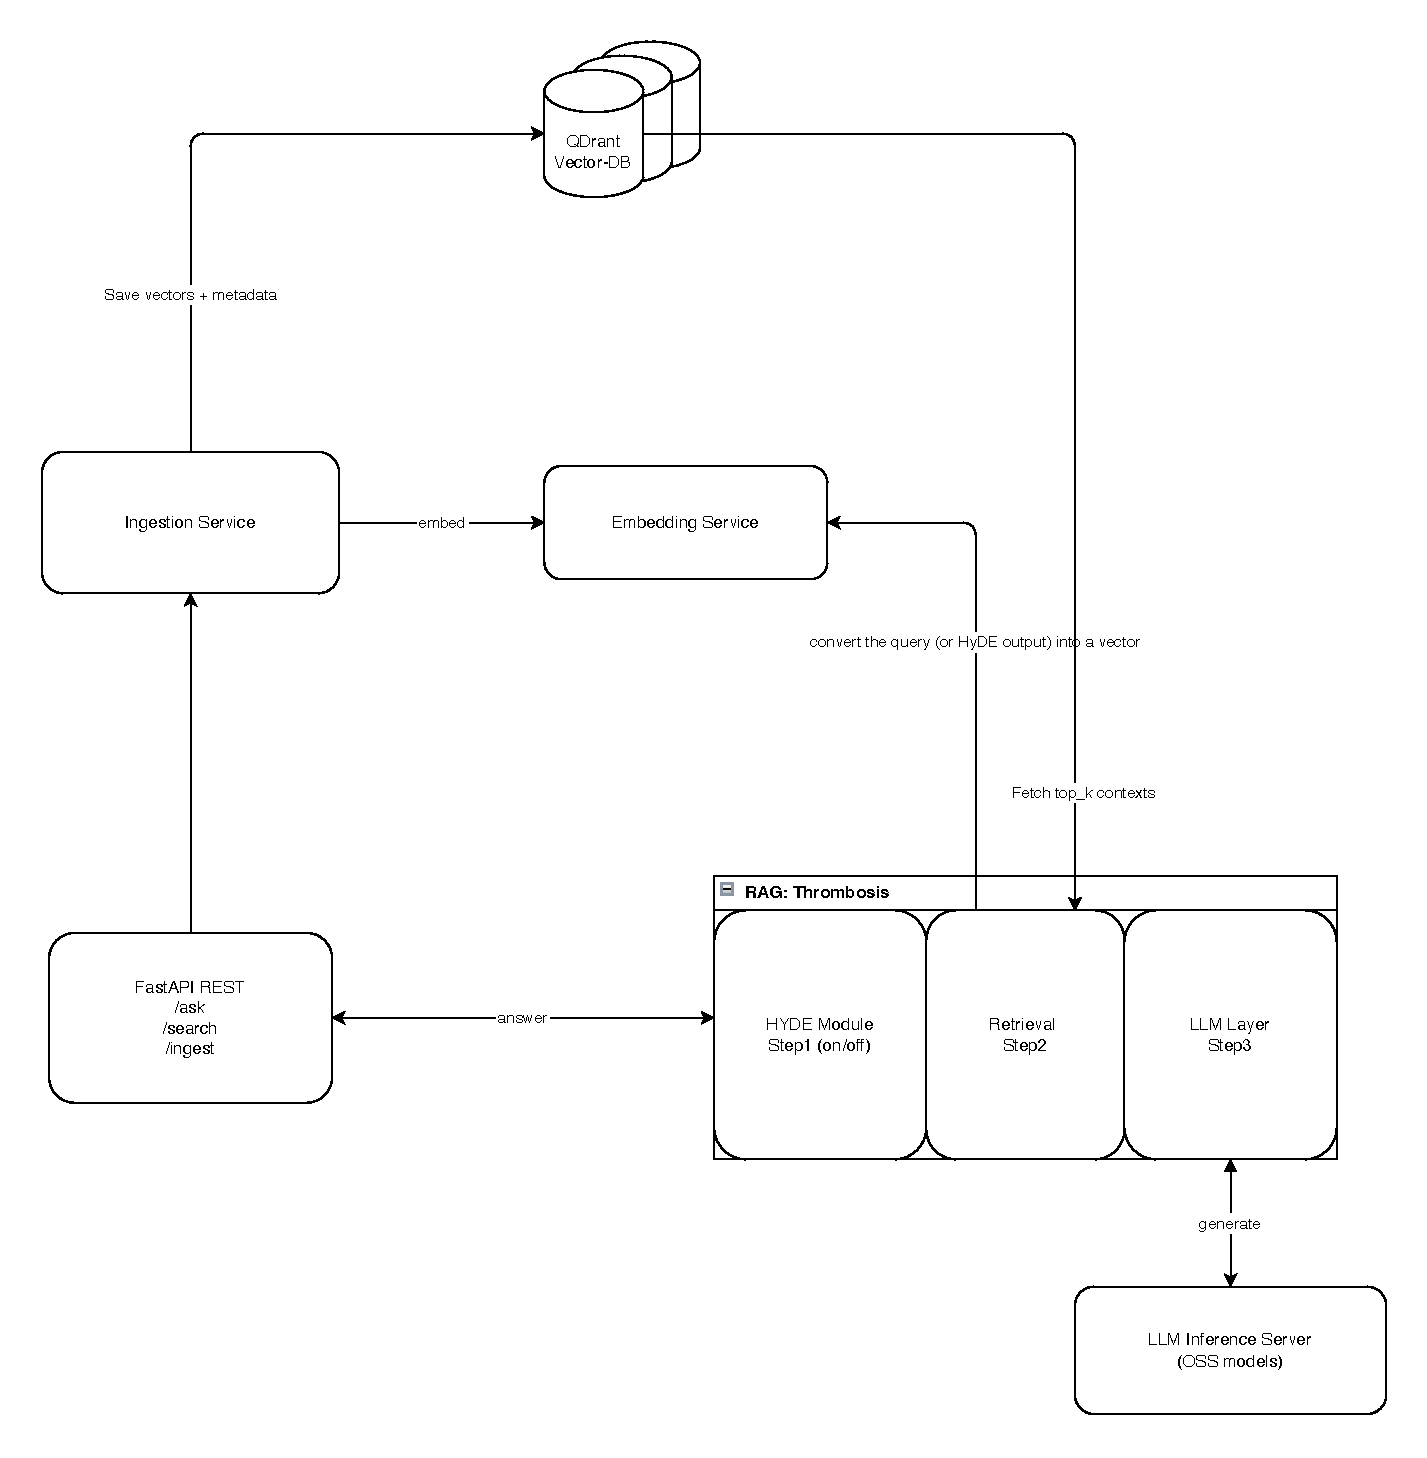
\includegraphics[width=0.9\linewidth]{resources/images/HLD.pdf}
\caption{High level architecture of the platform.}
\label{fig:architecture-high-level}
\end{figure}

Figure~\ref{fig:architecture-high-level} summarizes this decomposition and highlights a key design decision: scheduler execution and query-serving execution are operationally decoupled. This limits failure propagation across subsystems, but introduces eventual consistency between newly acquired literature and immediately retrievable indexed content.

\subsection{Subsystem Boundaries}

The high-level topology also reflects a contract-oriented integration strategy. The scheduler does not directly manipulate vector storage; instead, it communicates with the biomedical RAG service through documented endpoints for document existence checks, batch fetch, and ingest-job status tracking. This preserves ownership boundaries and reduces cross-service schema leakage, at the cost of additional network round-trips and stricter interface-version management.
% evidence: scheduler_pubmed/src/adapters/rag/documents_client.py
% evidence: scheduler_pubmed/src/core/ports/documents_client.py
% evidence: biomed_knowledge_platform/src/biomed_platform/api/endpoints/documents.py
% evidence: biomed_knowledge_platform/src/biomed_platform/api/endpoints/ingestion.py

\section{Human-in-the-Loop Curation Subsystem}

Label Studio is positioned in this architecture as a human-in-the-loop curation subsystem rather than as a core retrieval or answer-generation service. Its role is to host clinician-facing review tasks derived from candidate biomedical abstracts, while the surrounding \texttt{labelstudio-tools} package prepares tasks for upload, exports reviewed tasks, enriches them with bibliographic metadata, and hands curated records to the biomedical RAG ingestion API. This placement preserves a clean separation between evidence curation and online retrieval, while still allowing curated judgments to influence what enters the indexed corpus and what can later be used for evaluation-oriented analysis.
% evidence: labelstudio-tools/src/app/python/main.py
% evidence: labelstudio-tools/src/app/python/uploader.py
% evidence: labelstudio-tools/src/app/python/download_data/main.py
% evidence: labelstudio-tools/src/app/python/rag_importer/rag_integration.py

Architecturally, this subsystem sits between manual biomedical validation and downstream ingestion. Upstream, Excel-based abstract collections are loaded, optional exclusion filters are applied, and valid rows are transformed into Label Studio task payloads containing at minimum PMID, title, and abstract fields. Downstream, exported tasks are enriched with DOI and source metadata, partitioned into clean and rejected datasets according to ingestion requirements, and then transformed into batch ingestion requests for the biomedical RAG service. The resulting workflow constrains human review to a dedicated curation surface while keeping ingestion contracts explicit and machine-verifiable.
% evidence: labelstudio-tools/src/app/python/data_loader.py
% evidence: labelstudio-tools/src/app/python/filters.py
% evidence: labelstudio-tools/src/app/python/tasks.py
% evidence: labelstudio-tools/src/app/python/download_data/doi_enrich_any.py
% evidence: labelstudio-tools/src/app/python/download_data/main.py
% evidence: labelstudio-tools/src/app/python/rag_importer/rag_integration.py

This curation layer also has methodological significance for later evaluation chapters. The exported task structure retains manual annotation content alongside bibliographic identifiers and enriched metadata, which means curated tasks can act as traceable review artifacts rather than transient operator notes. At the same time, the current implementation validates metadata completeness for ingestion, but does not itself enforce annotation completeness or inter-annotator agreement constraints. The architectural tradeoff is therefore pragmatic: the subsystem increases traceability and enables clinician-informed dataset refinement, yet stronger annotation-governance guarantees remain an external workflow responsibility rather than a property enforced entirely in code.
% evidence: labelstudio-tools/ls_data/tasks_raw.json
% evidence: labelstudio-tools/src/app/python/download_data/main.py

\section{Component Architecture of the Biomedical RAG Service}

The biomedical RAG service is organized around four conceptual components: ingestion, retrieval, synthesis, and document management. The ingestion component accepts normalized document payloads, enforces duplicate constraints, and orchestrates asynchronous indexing. The retrieval component transforms user questions into vector-space candidates and assembles context-bearing evidence. The synthesis component produces structured answers with explicit citations. The document management component provides lifecycle controls required for lookup, verification, and deletion.
% evidence: biomed_knowledge_platform/src/biomed_platform/core/use_cases/ingestion.py
% evidence: biomed_knowledge_platform/src/biomed_platform/core/use_cases/search.py
% evidence: biomed_knowledge_platform/src/biomed_platform/core/use_cases/ask.py
% evidence: biomed_knowledge_platform/src/biomed_platform/core/use_cases/document_lookup.py
% evidence: biomed_knowledge_platform/src/biomed_platform/core/use_cases/delete_document.py

Architecturally, the service applies Clean Architecture with a ports-and-adapters realization. The API layer performs transport and schema duties, use cases orchestrate business workflows, the domain layer holds framework-independent models, and adapters implement infrastructure integrations behind abstract ports. Dependency direction is inward: outer layers depend on inner policies through interfaces, while the domain remains independent of frameworks and vendors. This structure improves maintainability through low coupling and supports reproducibility by making workflow behavior explicit at use-case boundaries.
% evidence: biomed_knowledge_platform/src/biomed_platform/core/ports/ingestion.py
% evidence: biomed_knowledge_platform/src/biomed_platform/core/ports/retrieval.py
% evidence: biomed_knowledge_platform/src/biomed_platform/core/ports/pubmed.py
% evidence: biomed_knowledge_platform/src/biomed_platform/core/ports/llm.py
% evidence: biomed_knowledge_platform/src/biomed_platform/api/endpoints/ingestion.py
% evidence: biomed_knowledge_platform/src/biomed_platform/core/use_cases/ingestion.py
% evidence: biomed_knowledge_platform/src/biomed_platform/core/domains/ingestion.py
% evidence: biomed_knowledge_platform/src/biomed_platform/adapters/qdrant/vector_index.py
% evidence: biomed_knowledge_platform/src/biomed_platform/adapters/pubmed/pubmed_client.py
% evidence: biomed_knowledge_platform/src/biomed_platform/adapters/ollama/ollama_client.py

\subsection{Dependency Direction and Encapsulation}

Within this structure, request lifecycle management is explicitly layered. Middleware components provide request identifiers, access logging, and audit capture before and after endpoint execution, while use cases handle domain-specific validation and orchestration. This partition clarifies operational accountability by separating cross-cutting concerns from business flow logic.
% evidence: biomed_knowledge_platform/src/biomed_platform/common/middleware/request_context.py
% evidence: biomed_knowledge_platform/src/biomed_platform/common/middleware/audit.py
% evidence: biomed_knowledge_platform/src/biomed_platform/api/app.py

The scheduler service follows the same architectural approach with its own API, domain, use-case, adapter, and repository layers. This symmetry reduces conceptual overhead when reasoning about cross-service workflows and facilitates consistent error and status semantics between ingestion-oriented and acquisition-oriented operations.
% evidence: scheduler_pubmed/src/api/app.py
% evidence: scheduler_pubmed/src/core/domains/scheduler.py
% evidence: scheduler_pubmed/src/core/use_cases/scheduler.py
% evidence: scheduler_pubmed/src/db/repositories/scheduler_repository.py

\section{Scheduler Architecture and Continuous Literature Acquisition}

The scheduler service exists to convert irregular manual updates into controlled continuous literature acquisition. Its architecture persists query definitions, creates run records, and stores per-query and per-document outcomes to maintain historical accountability of acquisition behavior.
% evidence: scheduler_pubmed/src/core/domains/pubmed_query.py
% evidence: scheduler_pubmed/src/core/domains/scheduler.py
% evidence: scheduler_pubmed/src/core/ports/scheduler_repository.py

Execution is intentionally asynchronous. Trigger operations start runs rapidly, while background tasks perform PubMed search, incremental filtering, duplicate checks against existing indexed documents, and downstream ingestion coordination. This decision reduces control-plane latency and improves operational resilience under network variability, while requiring explicit run tracking to observe completion.
% evidence: scheduler_pubmed/src/core/services/scheduler_runtime.py
% evidence: scheduler_pubmed/src/core/use_cases/scheduler.py
% evidence: scheduler_pubmed/src/adapters/pubmed/query_client.py
% evidence: scheduler_pubmed/src/adapters/rag/documents_client.py

Continuous acquisition is implemented as a constrained workflow rather than unconstrained crawling. The service resolves DOI candidates from PubMed responses and uses previous successful execution timestamps to support incremental acquisition semantics when publication metadata is available. This improves freshness-efficiency balance, but remains sensitive to upstream metadata incompleteness.
% evidence: scheduler_pubmed/src/core/use_cases/scheduler.py
% evidence: scheduler_pubmed/src/adapters/pubmed/query_client.py

Status derivation in scheduler execution is also explicit at both query and run levels. Query-level outcomes are computed from DOI-resolution and DOI-failure counts, while run-level outcomes are aggregated from query outcomes. This design improves interpretability of partial-success scenarios and avoids conflating upstream retrieval gaps with downstream ingestion errors.
% evidence: scheduler_pubmed/src/core/use_cases/scheduler.py
% evidence: scheduler_pubmed/src/core/domains/scheduler.py

\section{Document Lifecycle and Processing Pipeline}

The lifecycle begins when a document is introduced through direct ingestion requests or scheduler-initiated fetch requests. At acquisition time, requests can be resolved by Digital Object Identifier (DOI) or PubMed Identifier (PMID); however, the indexing identity in the retrieval store is DOI-centered through normalized DOI to document identifier transformation.
% evidence: biomed_knowledge_platform/src/biomed_platform/api/endpoints/ingestion.py
% evidence: biomed_knowledge_platform/src/biomed_platform/api/endpoints/documents.py
% evidence: biomed_knowledge_platform/src/biomed_platform/core/use_cases/document_fetch.py
% evidence: biomed_knowledge_platform/src/biomed_platform/common/utils.py
% evidence: biomed_knowledge_platform/src/biomed_platform/core/use_cases/ingestion.py

Processing proceeds through asynchronous ingestion jobs. The architecture validates candidate items, reserves document identities to prevent conflicting writes, persists payload state, and dispatches workers for chunking, embedding, and vector indexing. Section-aware chunking and payload preservation ensure that downstream retrieval can reconstruct coherent evidence segments with provenance-bearing metadata.
% evidence: biomed_knowledge_platform/src/biomed_platform/core/use_cases/ingestion.py
% evidence: biomed_knowledge_platform/src/biomed_platform/core/services/ingestion/worker.py
% evidence: biomed_knowledge_platform/src/biomed_platform/core/services/ingestion/chunking.py
% evidence: biomed_knowledge_platform/src/biomed_platform/core/services/ingestion/pipeline.py

This pipeline prioritizes bounded request latency and operational recoverability over immediate index visibility. The tradeoff is eventual indexing completion, which requires explicit job polling for deterministic lifecycle observation.
% evidence: biomed_knowledge_platform/src/biomed_platform/api/endpoints/ingestion.py
% evidence: biomed_knowledge_platform/src/biomed_platform/core/domains/ingestion.py

Duplicate control is handled in two complementary layers: request-level idempotency keys and document-level reservation/commit semantics. This two-layer strategy mitigates duplicate writes arising from client retries and concurrent ingestion attempts. The tradeoff is additional state management overhead, including time-to-live policies for idempotency and payload stores.
% evidence: biomed_knowledge_platform/src/biomed_platform/core/services/ingestion/in_memory_idempotency.py
% evidence: biomed_knowledge_platform/src/biomed_platform/core/services/ingestion/vector_index_document_registry.py
% evidence: biomed_knowledge_platform/src/biomed_platform/core/services/ingestion/in_memory_payload_store.py

\section{Retrieval and Answer Generation Pipeline}

The retrieval pipeline transforms a user question into a ranked evidence context. Query embeddings are generated, vector candidates are retrieved under optional constraints, and candidate sets are reduced to bounded context windows before synthesis. This architecture constrains unbounded prompt growth and supports consistent runtime behavior under configurable limits.
% evidence: biomed_knowledge_platform/src/biomed_platform/core/use_cases/search.py
% evidence: biomed_knowledge_platform/src/biomed_platform/core/use_cases/ask.py
% evidence: biomed_knowledge_platform/src/biomed_platform/core/services/hallucination/synthesis.py

The synthesis stage uses an LLM to generate structured responses with explicit citation linkage to retrieved context. An optional retrieval expansion mode, Hypothetical Document Embeddings (HyDE), generates a hypothetical passage from the question, embeds it, and merges those candidates with direct-question candidates before reranking. The rationale is improved semantic recall for difficult or underspecified biomedical questions. The tradeoff is increased dependency on generation quality and higher response-time variance.
% evidence: biomed_knowledge_platform/src/biomed_platform/core/use_cases/ask.py
% evidence: biomed_knowledge_platform/src/biomed_platform/core/services/hyde/hyde.py
% evidence: biomed_knowledge_platform/src/biomed_platform/core/services/hyde/hybrid_retrieval.py
% evidence: biomed_knowledge_platform/src/biomed_platform/core/domains/synthesis.py

The ask flow further constrains synthesis reliability through explicit limits on candidate chunks, final chunk selection, and context length. These limits bound prompt size and stabilize runtime behavior under heterogeneous document lengths. The architectural implication is a controlled tradeoff between context breadth and deterministic resource usage.
% evidence: biomed_knowledge_platform/src/biomed_platform/api/endpoints/ask.py
% evidence: biomed_knowledge_platform/src/biomed_platform/core/use_cases/ask.py
% evidence: biomed_knowledge_platform/src/biomed_platform/core/services/hallucination/synthesis.py

\section{Data and Persistence Architecture}

The persistence model combines operational state persistence and evaluation artifact persistence. Operationally, indexed chunk data and metadata are retained in the vector layer, while ingestion job states, duplicate-control records, and scheduler execution states are persisted to support lifecycle reconstruction and failure recovery. In the vector layer, per-chunk point identifiers are derived from document identifier and chunk index, and the document identifier is derived from normalized DOI, thereby enforcing a DOI-centered document identity model for retrieval and deletion workflows.
% evidence: biomed_knowledge_platform/src/biomed_platform/core/services/ingestion/pipeline.py
% evidence: biomed_knowledge_platform/src/biomed_platform/core/services/ingestion/in_memory_job_store.py
% evidence: biomed_knowledge_platform/src/biomed_platform/core/services/ingestion/in_memory_idempotency.py
% evidence: scheduler_pubmed/src/core/ports/scheduler_repository.py
% evidence: biomed_knowledge_platform/src/biomed_platform/common/utils.py
% evidence: biomed_knowledge_platform/src/biomed_platform/core/use_cases/document_lookup.py
% evidence: biomed_knowledge_platform/src/biomed_platform/core/use_cases/delete_document.py

For experimentation, the evaluation subsystem persists phase-specific artifacts, including retrieval pools, generated-answer outputs, and derived metric tables. The architectural implication is that experiment results remain inspectable as first-class outputs rather than transient logs. The tradeoff is increased artifact management burden across repeated runs.
% evidence: evaluation_metrics/src/phases/phase1_pool.py
% evidence: evaluation_metrics/src/phases/phase3_generate.py
% evidence: evaluation_metrics/src/phases/phase4_ragas.py
% evidence: evaluation_metrics/src/phases/phase6_extraction.py

This persistence strategy enables cross-phase diagnostic analysis. Retrieval outputs can be linked to subsequent answer-generation records, and those outputs can then be evaluated by dedicated metrics phases. The resulting provenance chain supports methodological scrutiny by preserving intermediate states that would otherwise be lost in end-only evaluation designs.
% evidence: evaluation_metrics/src/phases/phase1_pool.py
% evidence: evaluation_metrics/src/phases/phase3_generate.py
% evidence: evaluation_metrics/src/phases/phase5_audit.py

The evaluation approach is implemented as a command-line orchestration layer that materializes per-run directories and phase outputs, while external model-serving dependencies are supplied by a dedicated Ollama deployment stack. This separation ensures that evaluator configuration, run artifacts, and model-hosting lifecycle can be inspected independently when reproducing or auditing experiments.
% evidence: evaluation_metrics/src/eval_cli.py
% evidence: evaluation_metrics/src/clients/ollama_api.py
% evidence: llm_server/docker-compose.yml
% evidence: llm_server/ollama/init-models.sh

\section{Operational Observability}

Observability is designed as a reliability and validity mechanism. Health and readiness endpoints separate process liveness from dependency readiness, enabling conservative admission behavior under partial infrastructure degradation. This distinction is particularly important when vector, database, or generation dependencies fail independently.
% evidence: biomed_knowledge_platform/src/biomed_platform/api/endpoints/system.py
% evidence: biomed_knowledge_platform/src/biomed_platform/core/services/readiness.py
% evidence: scheduler_pubmed/src/api/endpoints/health.py

In parallel, request-context tracing and audit persistence provide reconstructable interaction histories, including request metadata, response status, and exception traces. The design improves post hoc diagnosis and experiment-time incident correlation. Its tradeoff is higher write overhead and stricter governance obligations for recorded payload content.
% evidence: biomed_knowledge_platform/src/biomed_platform/common/middleware/request_context.py
% evidence: biomed_knowledge_platform/src/biomed_platform/common/middleware/audit.py
% evidence: tests/bdd/features/audit.feature

\section{Architectural Limitations}

The architecture is constrained by external service behavior. Retrieval and synthesis quality depend on external model and infrastructure services beyond strict transactional control, while literature acquisition depends on upstream metadata fidelity. As a result, the system can provide explicit detection and recording of many failures, but cannot guarantee elimination of dependency-induced variance.

A second limitation is eventual consistency across acquisition and retrieval planes. Because acquisition and ingestion are asynchronous, recently identified documents may not be immediately available for retrieval. This is an intentional tradeoff that preserves bounded control-plane latency and operational isolation between serving and acquisition workflows.
% evidence: biomed_knowledge_platform/src/biomed_platform/core/services/ingestion/worker.py
% evidence: scheduler_pubmed/src/core/services/scheduler_runtime.py

Finally, reproducibility is strong at the workflow and artifact level but limited at the strict output-identity level for generation stages. Structured run artifacts and state transitions provide robust comparability across experiments, yet LLM-mediated synthesis can still exhibit output variation under equivalent high-level inputs.
% evidence: evaluation_metrics/src/phases/phase3_generate.py
% evidence: evaluation_metrics/src/phases/phase4_ragas.py

An additional limitation is sensitivity to identifier completeness in upstream biomedical sources. Scheduler-side DOI extraction and downstream document existence checks rely on consistent metadata availability; when identifiers are missing or inconsistently formatted, conservative failure or skip paths may reduce acquisition coverage for a given run window.
% evidence: scheduler_pubmed/src/adapters/pubmed/query_client.py
% evidence: scheduler_pubmed/src/core/use_cases/scheduler.py

\subsection{Architectural Tradeoffs Summary}

Taken together, the architecture favors explicit subsystem boundaries, inward dependency direction, and asynchronous workflow isolation to improve maintainability and reproducibility. The corresponding tradeoffs are eventual consistency, additional coordination overhead between services, and bounded but non-zero variance in LLM-mediated synthesis behavior.
